\documentclass{article}
\usepackage{graphicx} % Required for inserting images
\usepackage[section]{placeins}
\usepackage{amsmath}
\usepackage{subfig}
\usepackage{babel,blindtext}
\usepackage[section]{placeins}
\captionsetup{justification=raggedright,singlelinecheck=false}


\title{CS180 Project 2}
\author{Kyle Wong}
\date{September 2023}

\begin{document}

\maketitle

\section{Fun With Filters}
\subsection{Finite Difference Operator}
Gradient Magnitude image formula:\\
Dx = 
$\begin{bmatrix}
1 & -1
\end{bmatrix}$
\\
Dy = 
$\begin{bmatrix}
1\\
-1
\end{bmatrix}$\\
Dx\_im = Dx * image\\
Dy\_im = Dy * image\\
Gradient Magnitude = $\sqrt{Dx\_im ^2 + Dy\_im ^2}$\\

To calculate the partial derivative in x and y, I convolved the image with finite difference operators Dx and Dy. The Dx operator will do a basic slope calculation between the im[y, x] and im[y, x+1]. The Dy operator will do the same but in the y-axis. Important to note that the Dx will find vertical edges and the Dy will find horizontal edges. The gradient magnitude represents how we want the average of these changes therefore we just do the L\_2 Norm of Dx\_im and Dy\_in. There are many edges in the image, but we want just the prominent ones and not the noisy ones. To find the real edges without noise, I binarized the gradient magnitude by choosing an appropriate threshold.


\begin{figure}[!htb]
\minipage{0.45\textwidth}
    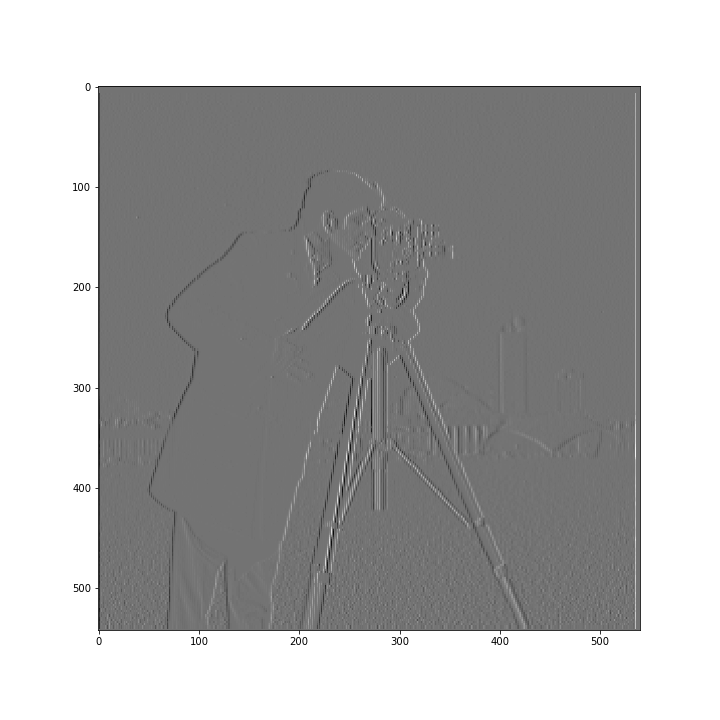
\includegraphics[width=\linewidth]{dx.png}
    \caption{dx}\label{fig:awesome_image1}
\endminipage
\minipage{0.45\textwidth}
    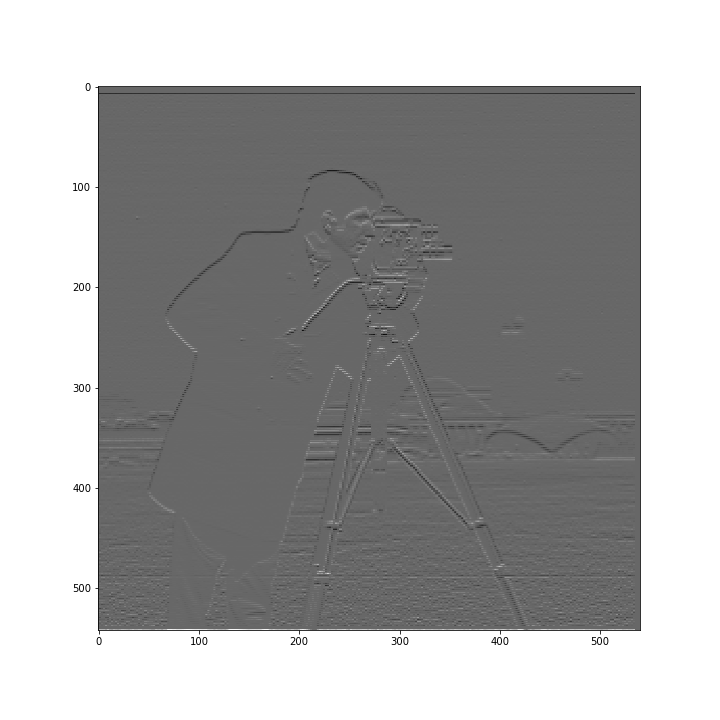
\includegraphics[width=\linewidth]{dy.png}
    \caption{dy}\label{fig:awesome_image2}
\endminipage

\minipage{0.45\textwidth}
    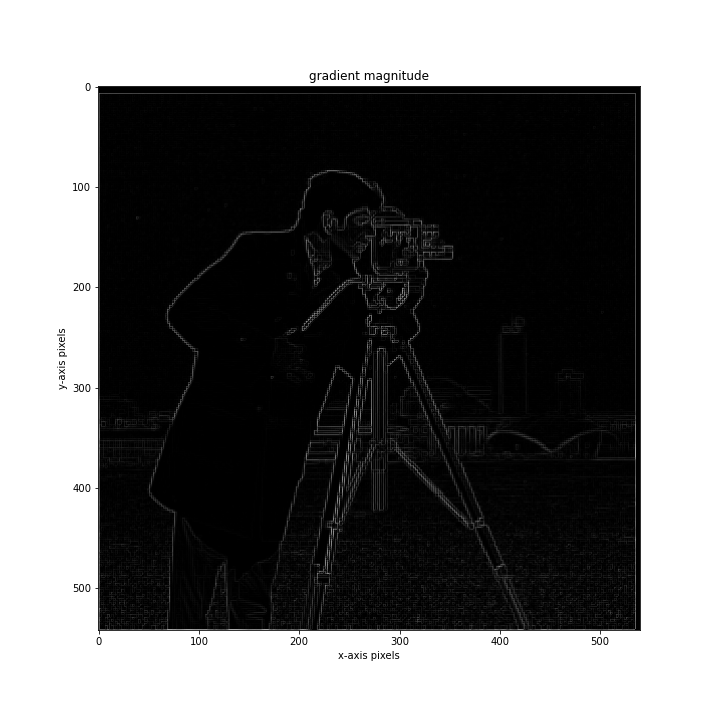
\includegraphics[width=\linewidth]{gradient magnitude.png}
    \caption{gradient magnitude}\label{fig:awesome_image1}
\endminipage
\minipage{0.45\textwidth}
    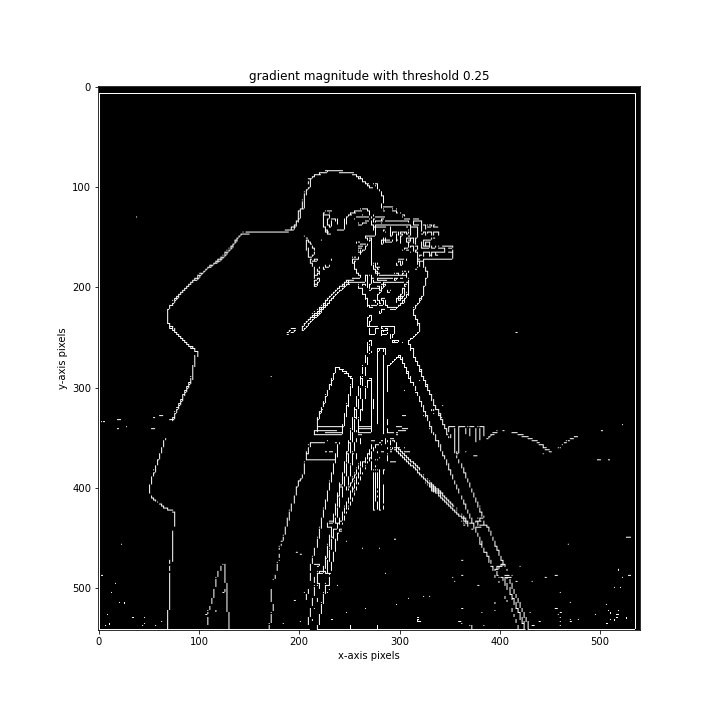
\includegraphics[width=\linewidth]{gradient magnitude threshold.png}
    \caption{gradient magnitude thres=0.25}\label{fig:awesome_image2}
\endminipage
\end{figure}
\FloatBarrier

\subsection{Derivative of Gaussian (DoG) Filter}
Differences between 1.1 and 1.2 (Gaussian blurring): In the blurred image, the edges are more prominent and there is less noise in the image. Since the high frequencies have been removed, the threshold value can be reduced since only the most prominent edges remain. In this case it went from 0.25 to 0.03.

The graphs "Blur then Derivative Convolve" and "Single Convolution" look basically the same with the prominent edges showing up in both of them.


\begin{figure}[!htb]
\minipage{0.45\textwidth}
    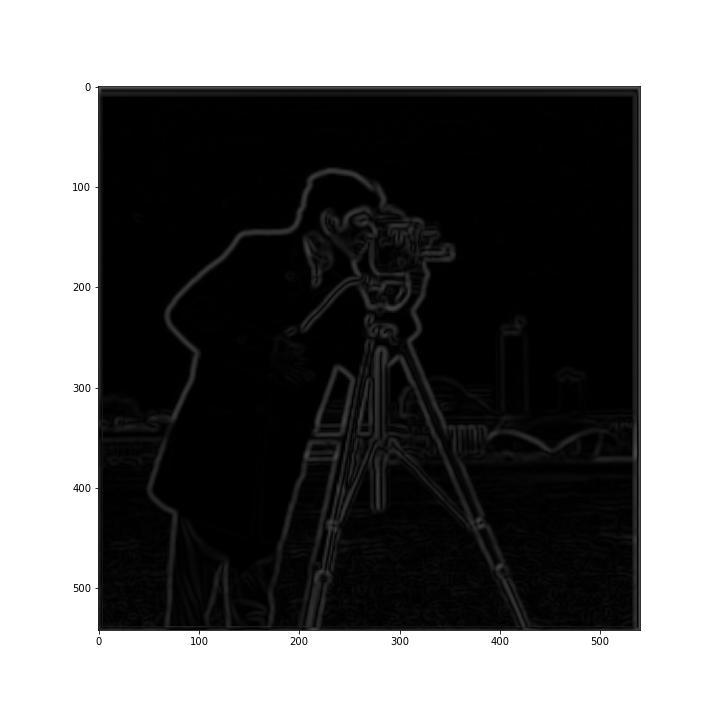
\includegraphics[width=\linewidth]{blur then convolve.png}
    \caption{blur then convolve}\label{fig:awesome_image1}
\endminipage
\minipage{0.45\textwidth}
    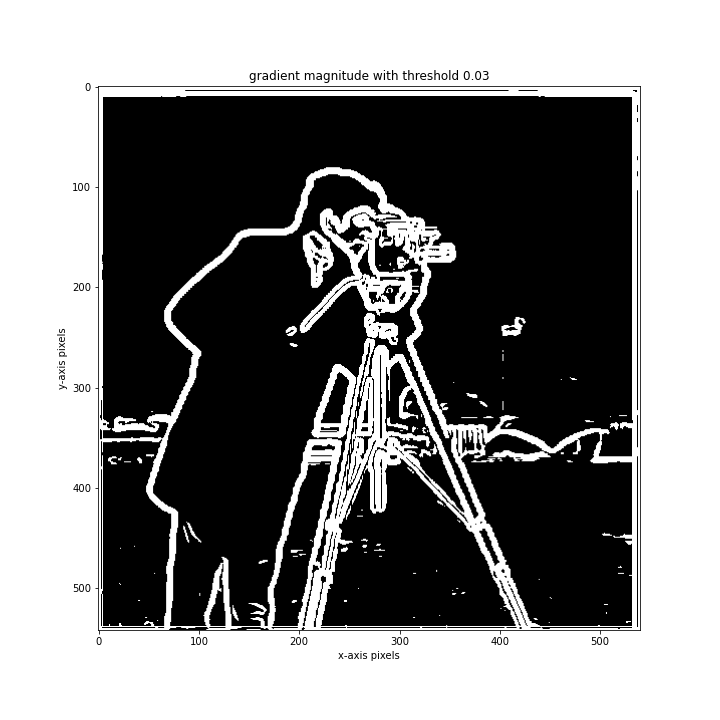
\includegraphics[width=\linewidth]{blur then convolve with threshold.png}
    \caption{blur then convolve thres=0.03}\label{fig:awesome_image2}
\endminipage

\minipage{0.45\textwidth}
    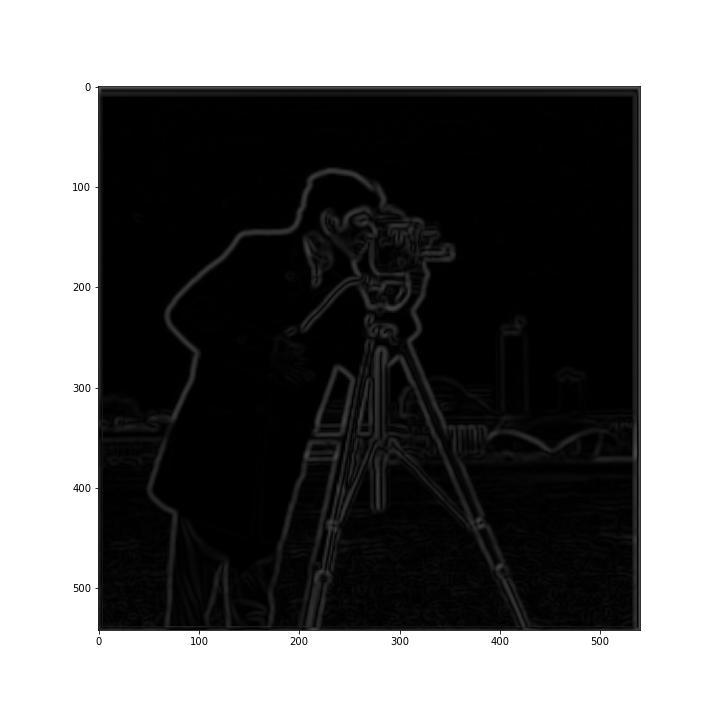
\includegraphics[width=\linewidth]{single convolution.png}
    \caption{single convolution}\label{fig:awesome_image1}
\endminipage
\minipage{0.45\textwidth}
    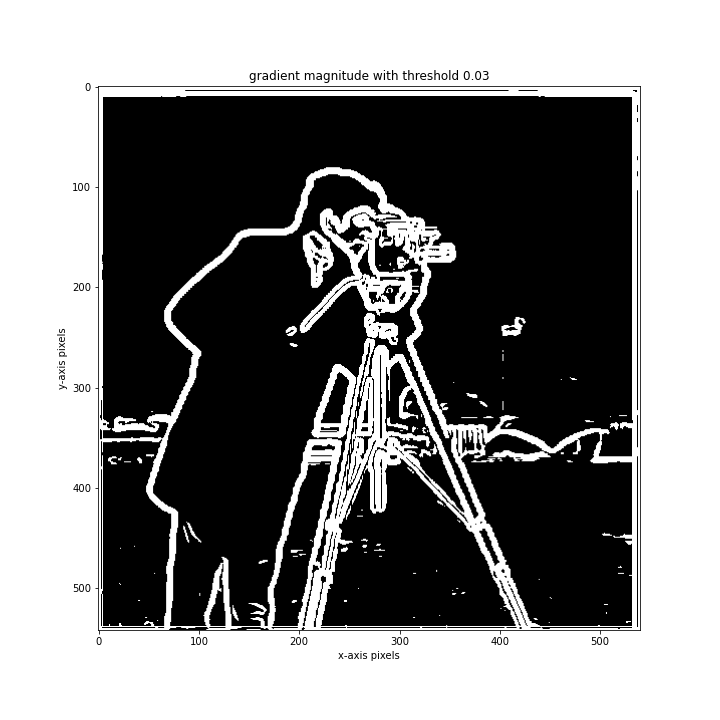
\includegraphics[width=\linewidth]{single convolution with threshold.png}
    \caption{single convolution thres=0.25}\label{fig:awesome_image2}
\endminipage
\end{figure}
\FloatBarrier


\section{Fun with Frequencies!}
\subsection{Image "Sharpening"}

\begin{figure}[!htb]
\minipage{0.45\textwidth}
    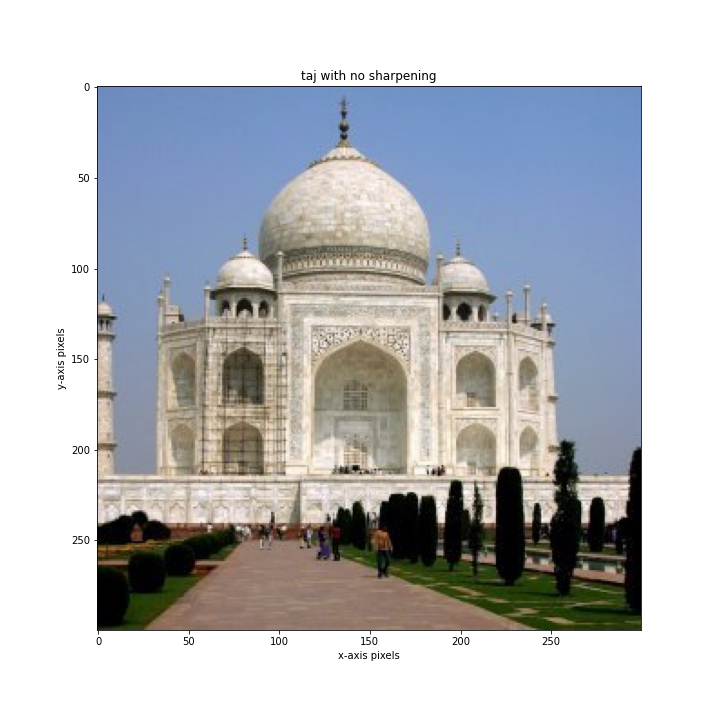
\includegraphics[width=\linewidth]{taj with no sharpening.png}
    \caption{taj with no sharpening}\label{fig:awesome_image1}
\endminipage
\minipage{0.45\textwidth}
    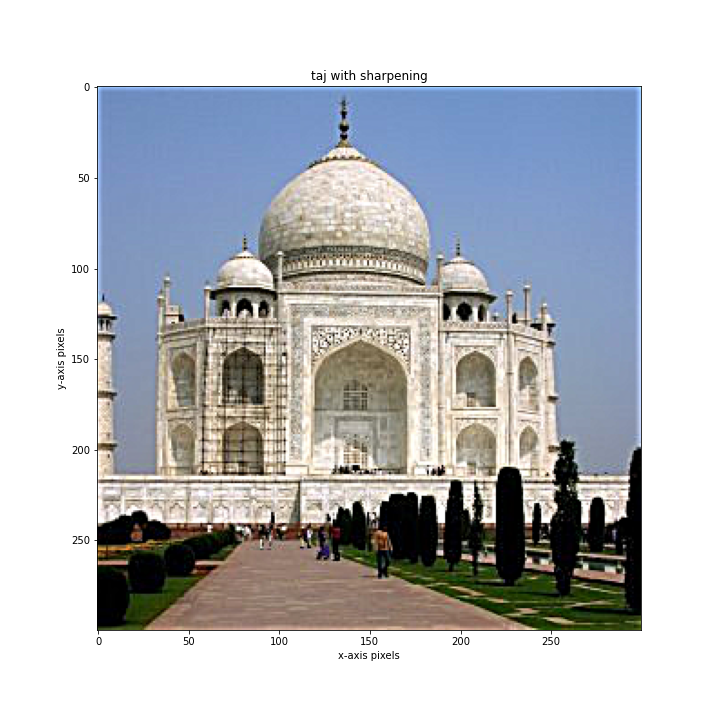
\includegraphics[width=\linewidth]{taj with sharpening.png}
    \caption{taj with sharpening}\label{fig:awesome_image2}
\endminipage
\end{figure}

\begin{figure}[!htb]
\minipage{0.45\textwidth}
    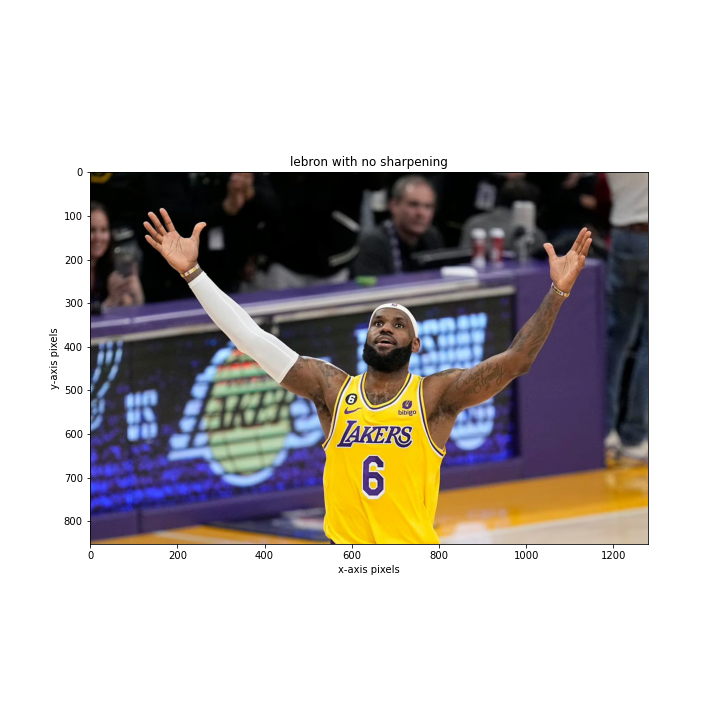
\includegraphics[width=\linewidth]{lebron with no sharpening.png}
    \caption{lebron with no sharpening}\label{fig:awesome_image1}
\endminipage
\minipage{0.45\textwidth}
    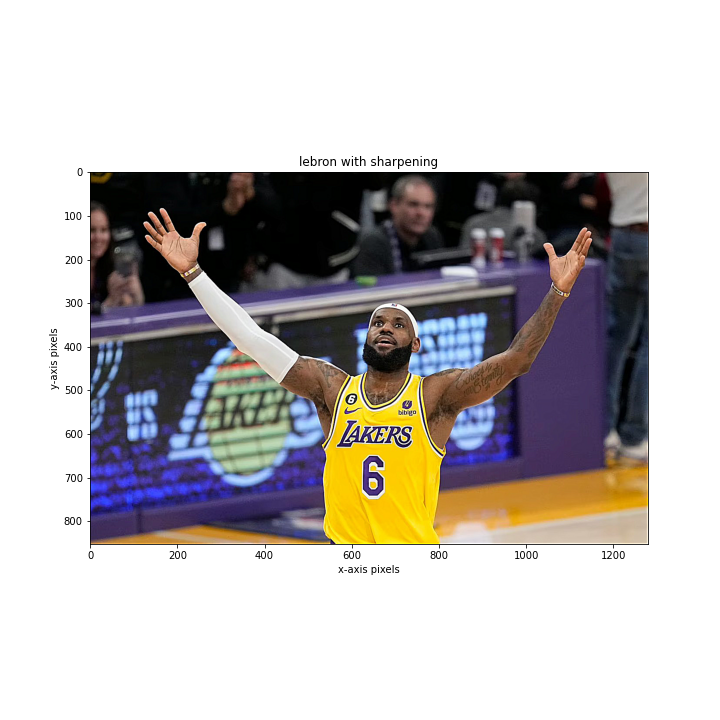
\includegraphics[width=\linewidth]{lebron with sharpening.png}
    \caption{lebron with sharpening}\label{fig:awesome_image2}
\endminipage
\end{figure}

\begin{figure}[!htb]
\minipage{0.45\textwidth}
    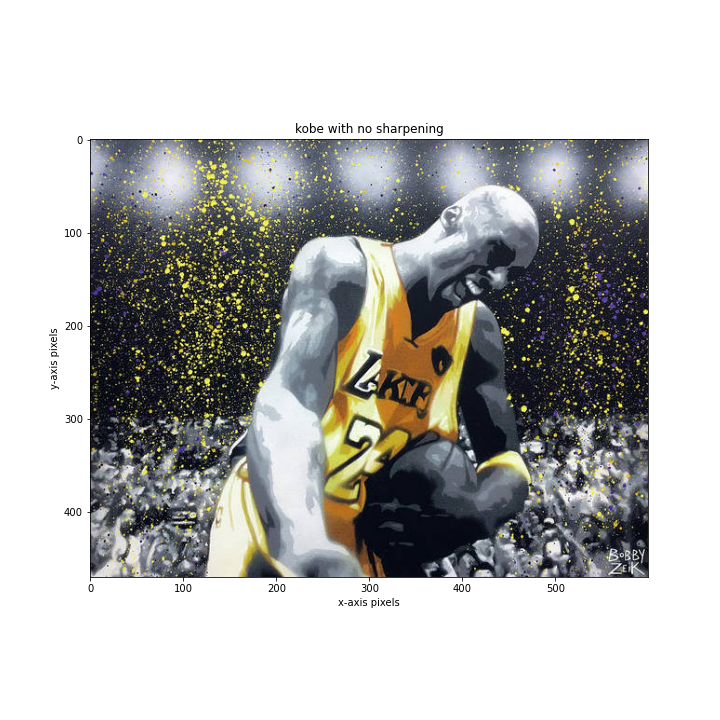
\includegraphics[width=\linewidth]{kobe with no sharpening.png}
    \caption{kobe with no sharpening}\label{fig:awesome_image1}
\endminipage
\minipage{0.45\textwidth}
    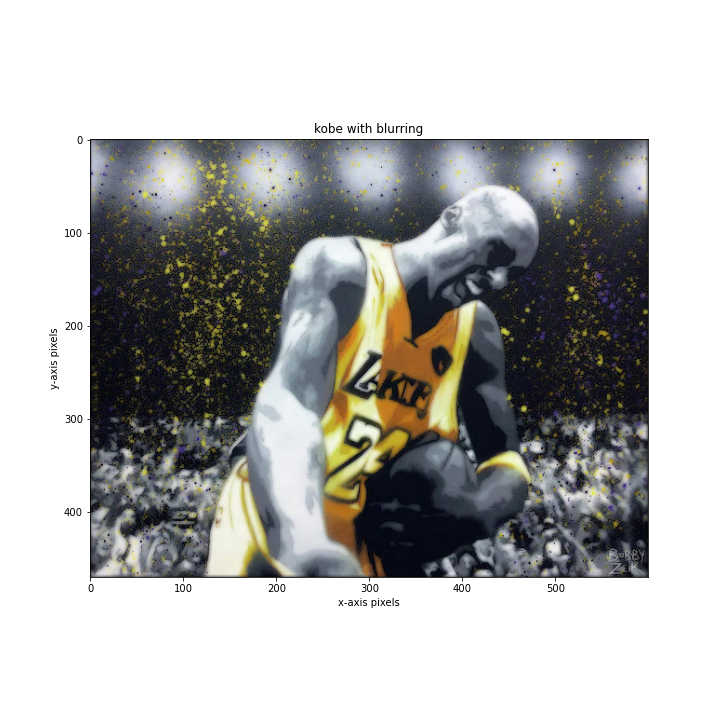
\includegraphics[width=\linewidth]{kobe with blurring.png}
    \caption{kobe with blurring}\label{fig:awesome_image2}
\endminipage
\minipage{0.45\textwidth}
    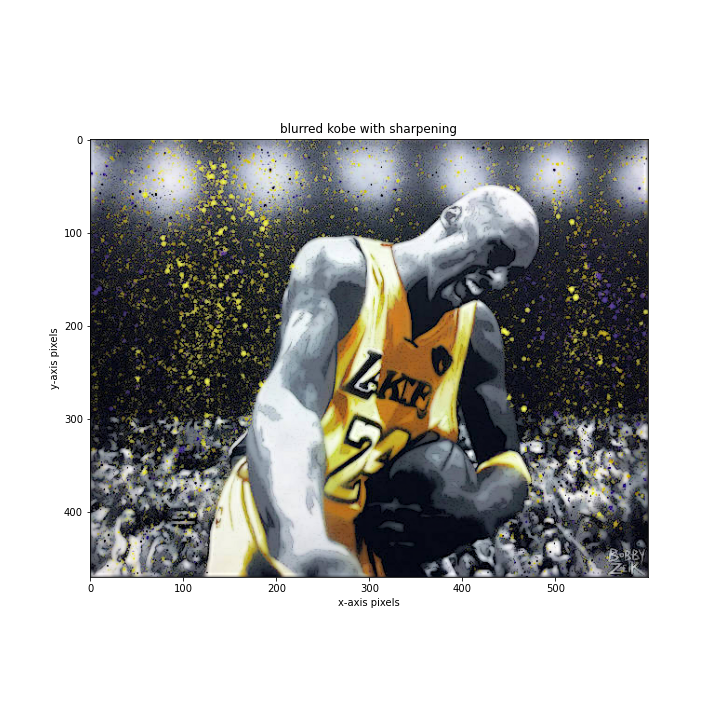
\includegraphics[width=\linewidth]{blurred kobe with sharpening.png}
    \caption{blurred kobe with sharpening}\label{fig:awesome_image2}
\endminipage
\end{figure}
\FloatBarrier

\subsection{Hybrid Images}
\begin{figure}[!htb]
\minipage{0.30\textwidth}
    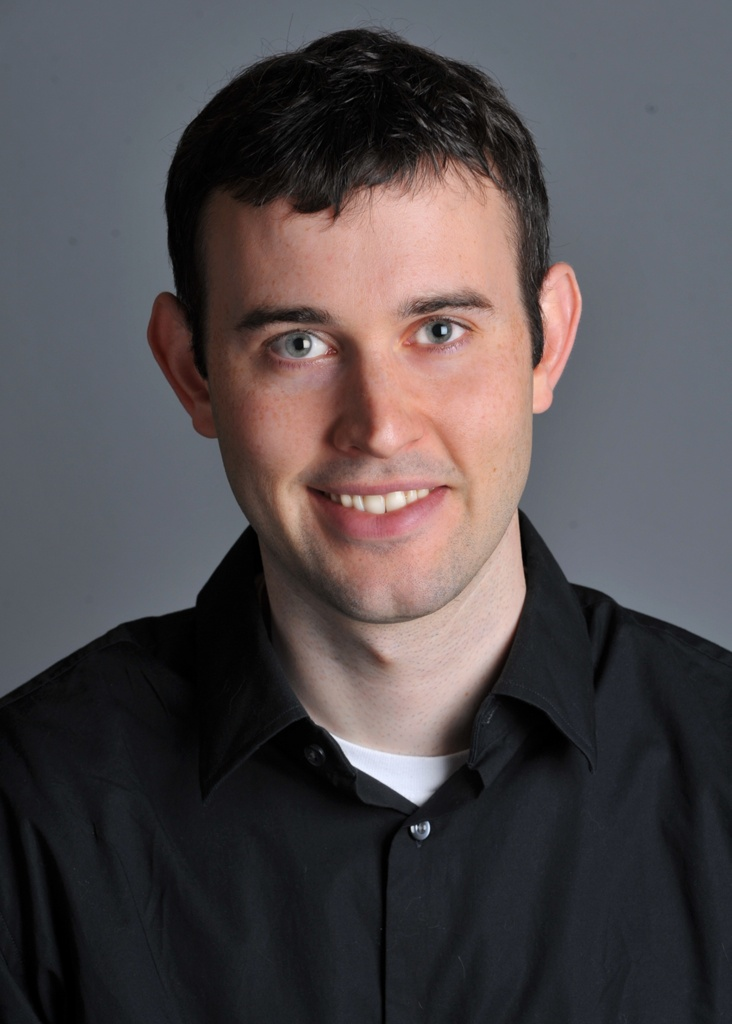
\includegraphics[width=\linewidth]{DerekPicture.jpg}
    \caption{Low Frequency Image In}\label{fig:awesome_image1}
\endminipage
\minipage{0.45\textwidth}
    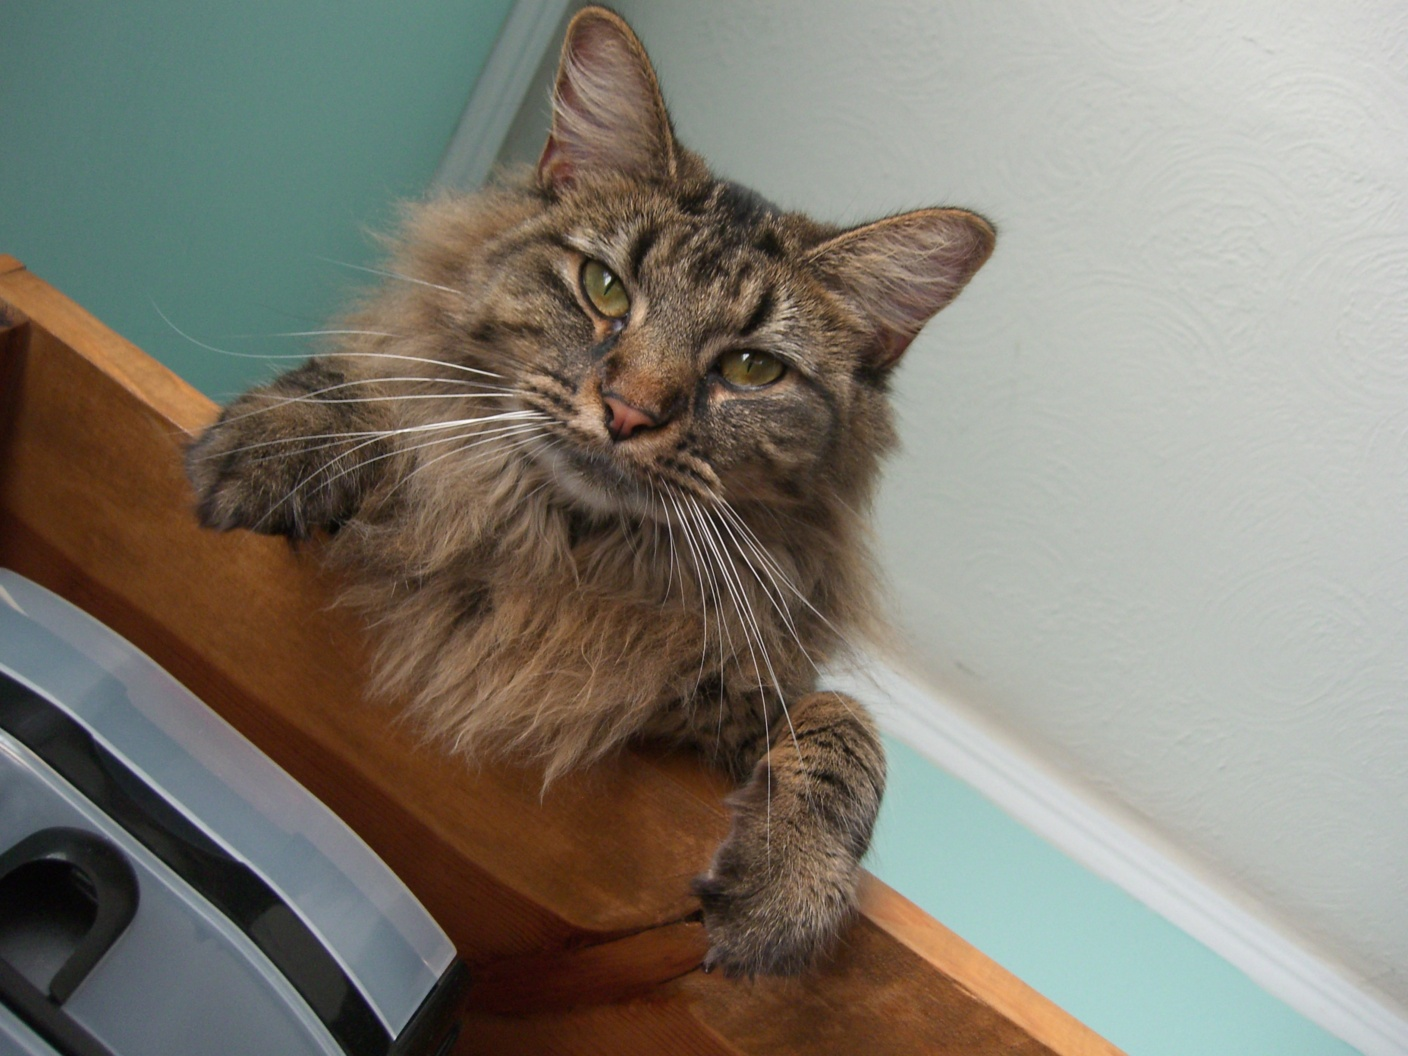
\includegraphics[width=\linewidth]{nutmeg.jpg}
    \caption{High Frequency Image In}\label{fig:awesome_image2}
\endminipage
\minipage{0.45\textwidth}
    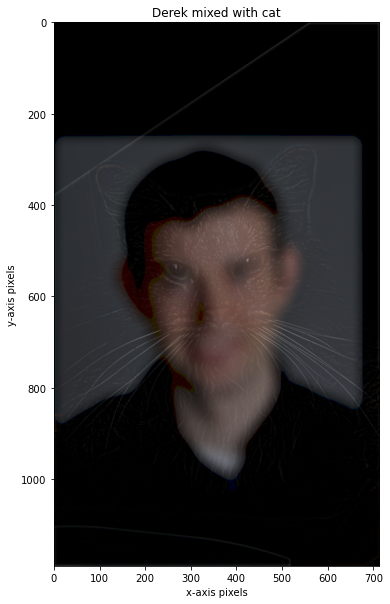
\includegraphics[width=\linewidth]{mancat.png}
    \caption{Hybrid}\label{fig:awesome_image2}
\endminipage
\end{figure}

\begin{figure}[!htb]
\title{\textbf {Failure}}
\paragraph{Failure: I had to bump the cat high frequencies up quite a bit for it to appear on the dog and it made the border appear. I did not know how to get rid of the border.}
\minipage{0.30\textwidth}
    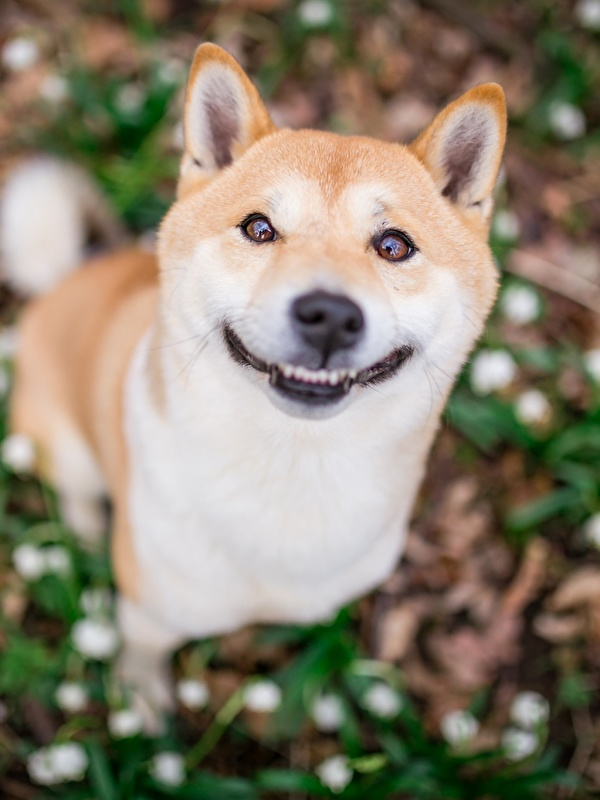
\includegraphics[width=\linewidth]{dog.jpeg}
    \caption{Low Frequency Image In}\label{fig:awesome_image1}
\endminipage
\minipage{0.30\textwidth}
    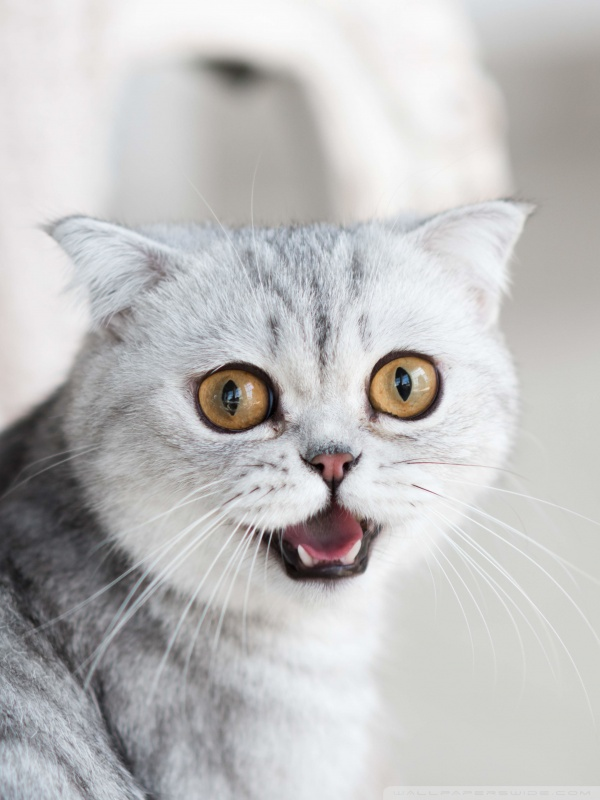
\includegraphics[width=\linewidth]{cat.jpeg}
    \caption{High Frequency Image In}\label{fig:awesome_image2}
\endminipage
\minipage{0.45\textwidth}
    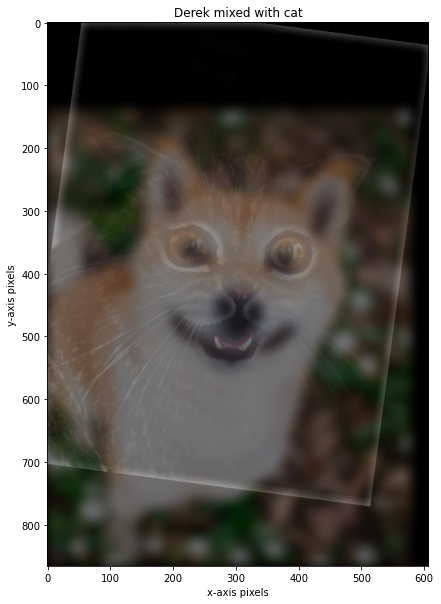
\includegraphics[width=\linewidth]{dogcat.png}
    \caption{Hybrid}\label{fig:awesome_image2}
\endminipage
\end{figure}

\begin{figure}[!htb]
\title{\textbf{Cat Evolution}}
\minipage{0.30\textwidth}
    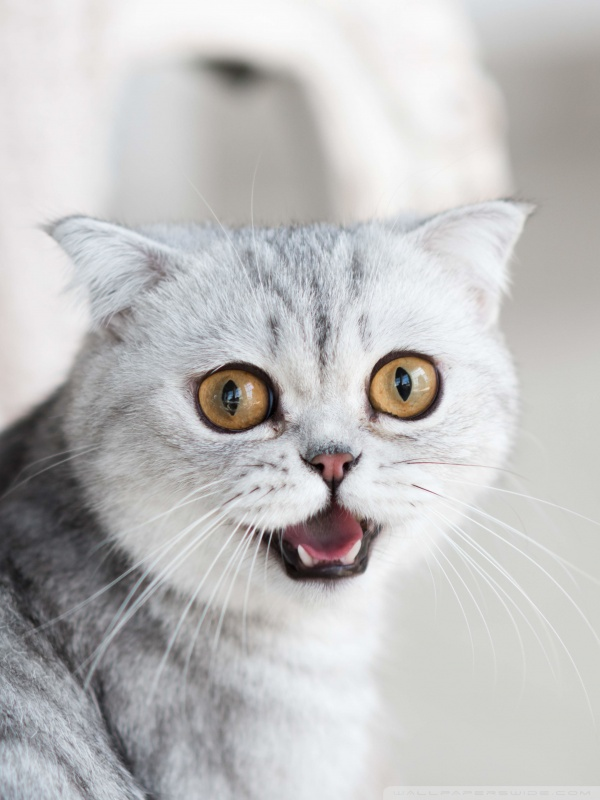
\includegraphics[width=\linewidth]{cat.jpeg}
    \caption{Low Frequency Image In}\label{fig:awesome_image1}
\endminipage
\minipage{0.30\textwidth}
    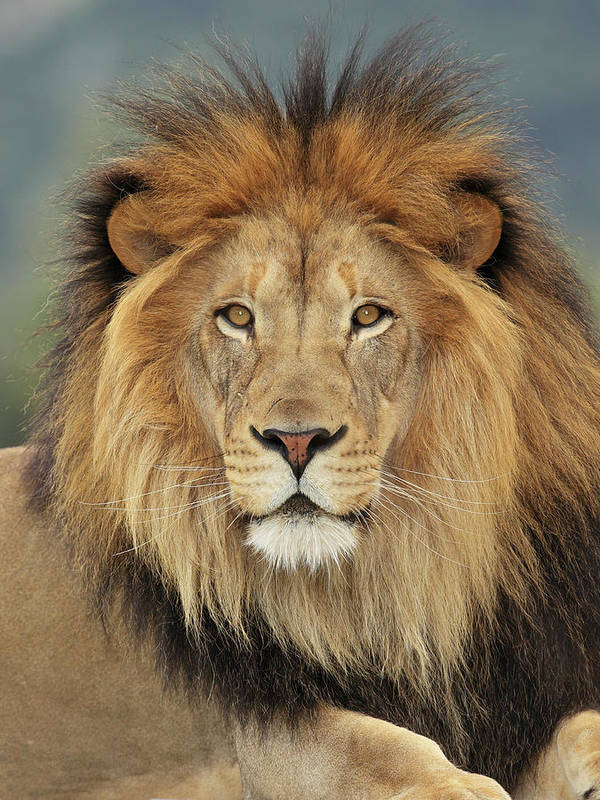
\includegraphics[width=\linewidth]{lion.jpeg}
    \caption{High Frequency Image In}\label{fig:awesome_image2}
\endminipage
\minipage{0.45\textwidth}
    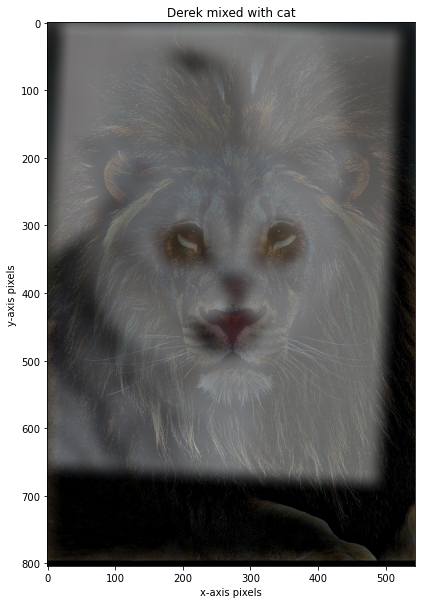
\includegraphics[width=\linewidth]{lioncat.png}
    \caption{Hybrid}\label{fig:awesome_image2}
\endminipage
\end{figure}

\begin{figure}[!htb]
\minipage{0.30\textwidth}
    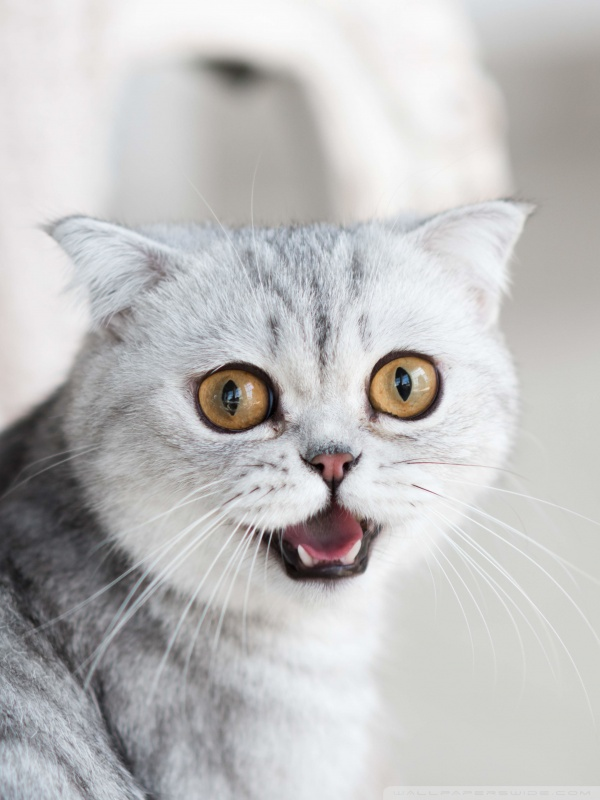
\includegraphics[width=\linewidth]{cat.jpeg}
    \caption{LF Image Input}\label{fig:awesome_image1}
\endminipage
\minipage{0.50\textwidth}
    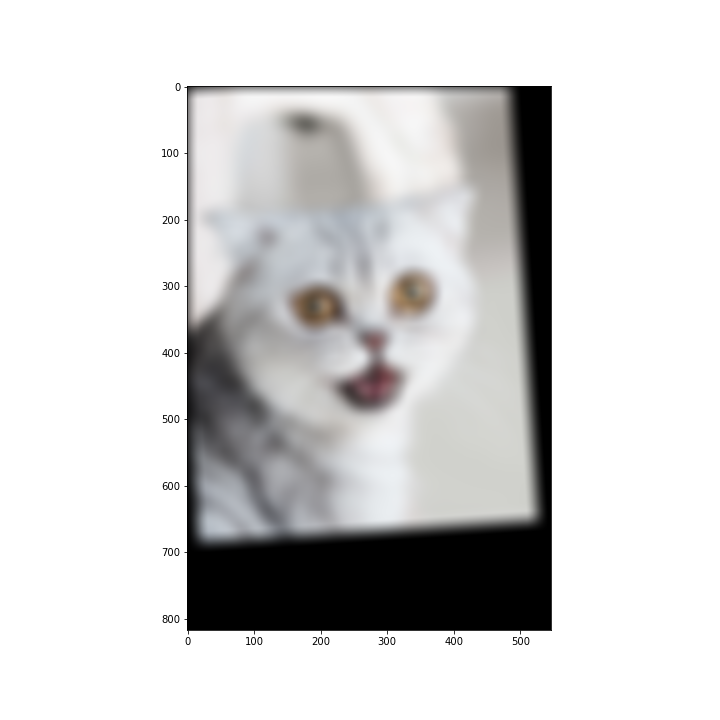
\includegraphics[width=\linewidth]{low cat.png}
    \caption{LF Image Low Frequencies Input}\label{fig:awesome_image2}
\endminipage
\minipage{0.75\textwidth}
    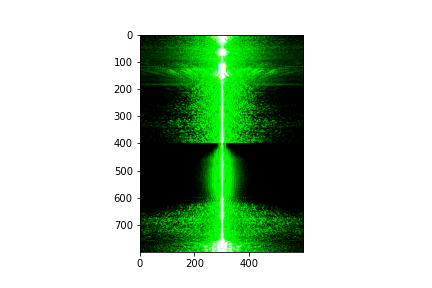
\includegraphics[width=\linewidth]{cat fourier.png}
    \caption{LF Image Input Low Freq FFT}\label{fig:awesome_image2}
\endminipage
\end{figure}

\begin{figure}[!htb]
\minipage{0.30\textwidth}
    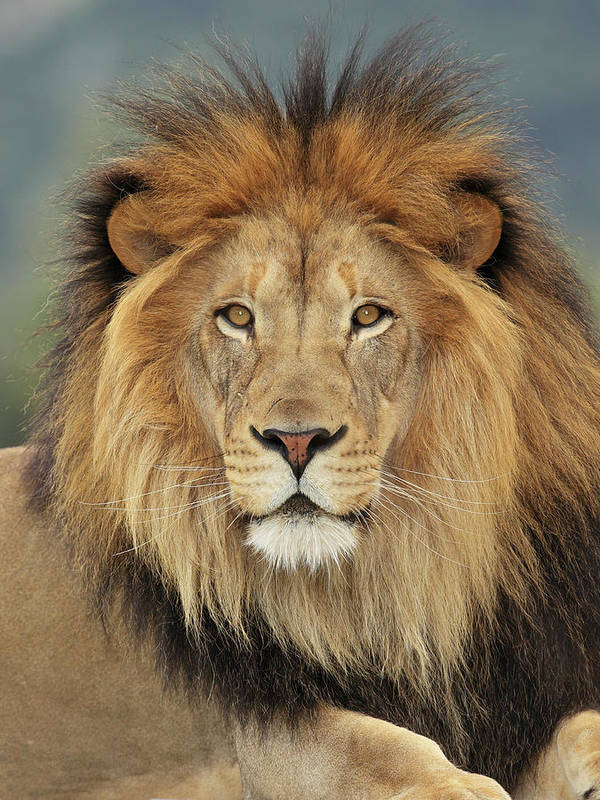
\includegraphics[width=\linewidth]{lion.jpeg}
    \caption{HF Image Input}\label{fig:awesome_image1}
\endminipage
\minipage{0.50\textwidth}
    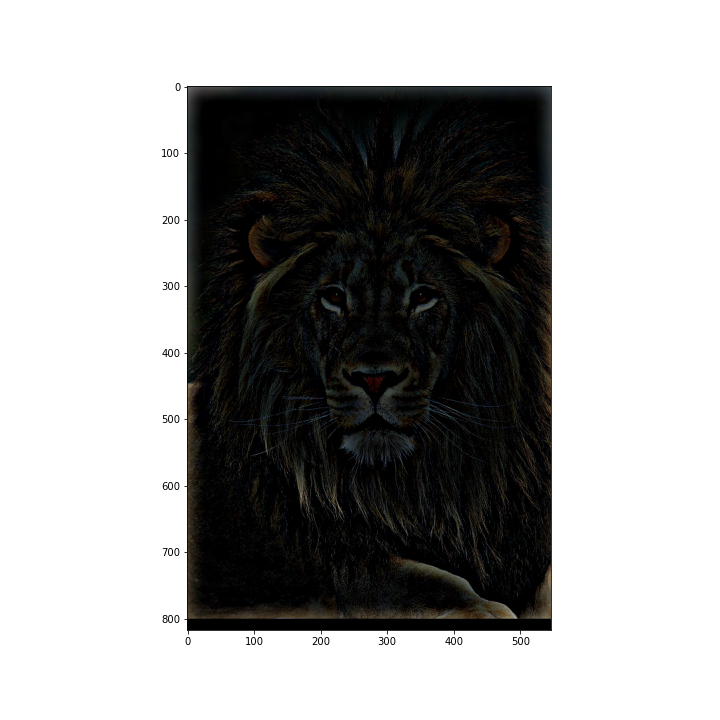
\includegraphics[width=\linewidth]{high lion.png}
    \caption{HF Image High Frequencies Input}\label{fig:awesome_image2}
\endminipage
\minipage{0.75\textwidth}
    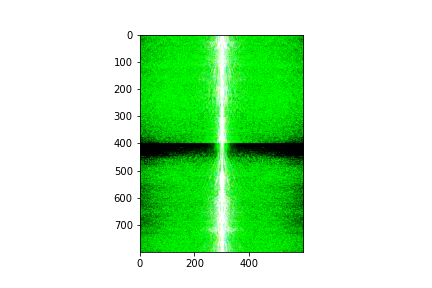
\includegraphics[width=\linewidth]{lion fourier.png}
    \caption{HF Image Input High Freq FFT}\label{fig:awesome_image2}
\endminipage
\end{figure}

\begin{figure}[!htb]
\minipage{0.75\textwidth}
    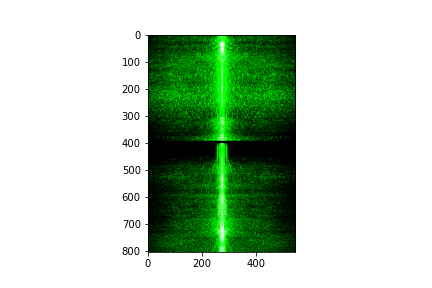
\includegraphics[width=\linewidth]{hybrid fourier.png}
    \caption{Hybrid Image FFT}\label{fig:awesome_image1}
\endminipage
\minipage{0.30\textwidth}
    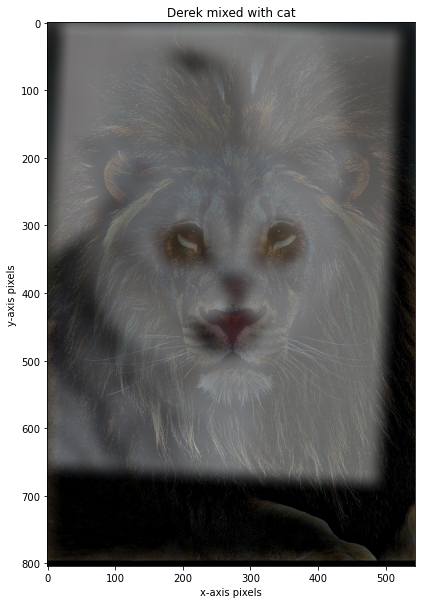
\includegraphics[width=\linewidth]{lioncat.png}
    \caption{Hybrid}\label{fig:awesome_image2}
\endminipage
\end{figure}
\FloatBarrier

\subsection{Gaussian and Laplacian Stacks}
\begin{figure}[!htb]
\title{apple gaussian}
\minipage{0.24\textwidth}
    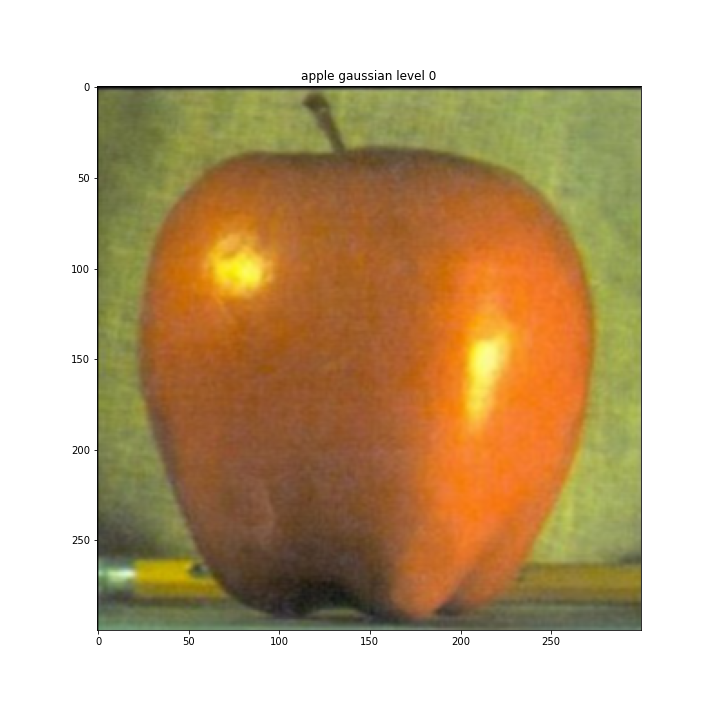
\includegraphics[width=\linewidth]{apple gaussian level 0.png}
\endminipage
\minipage{0.24\textwidth}
    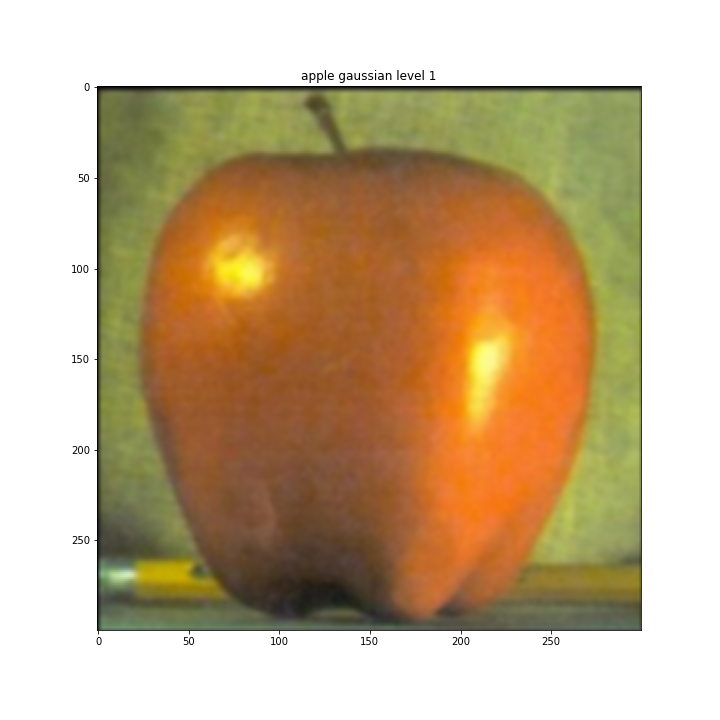
\includegraphics[width=\linewidth]{apple gaussian level 1.png}
\endminipage
\minipage{0.24\textwidth}
    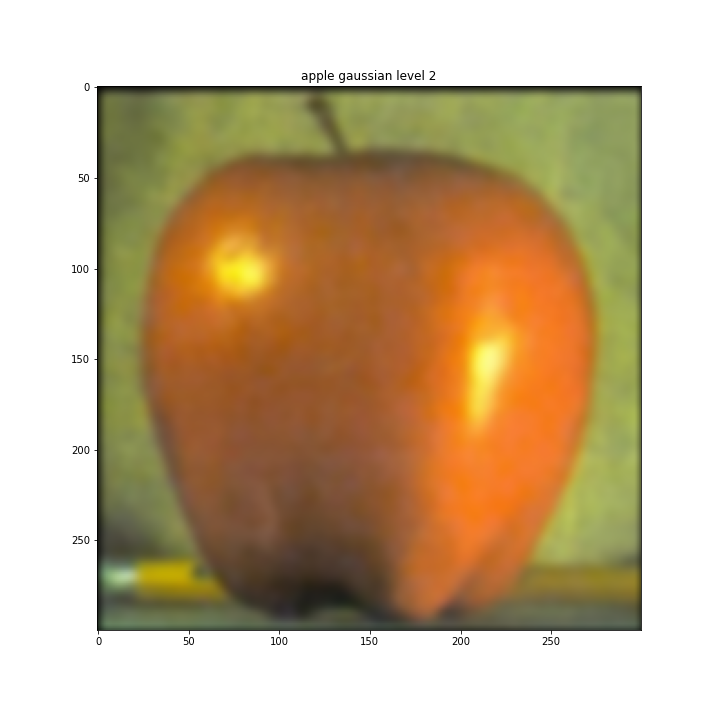
\includegraphics[width=\linewidth]{apple gaussian level 2.png}
\endminipage
\minipage{0.24\textwidth}
    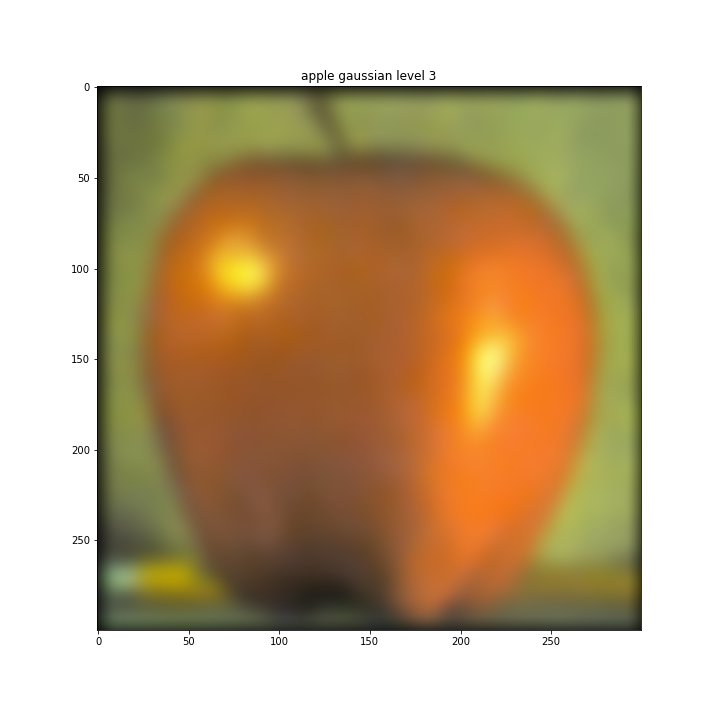
\includegraphics[width=\linewidth]{apple gaussian level 3.png}
\endminipage
\minipage{0.24\textwidth}
    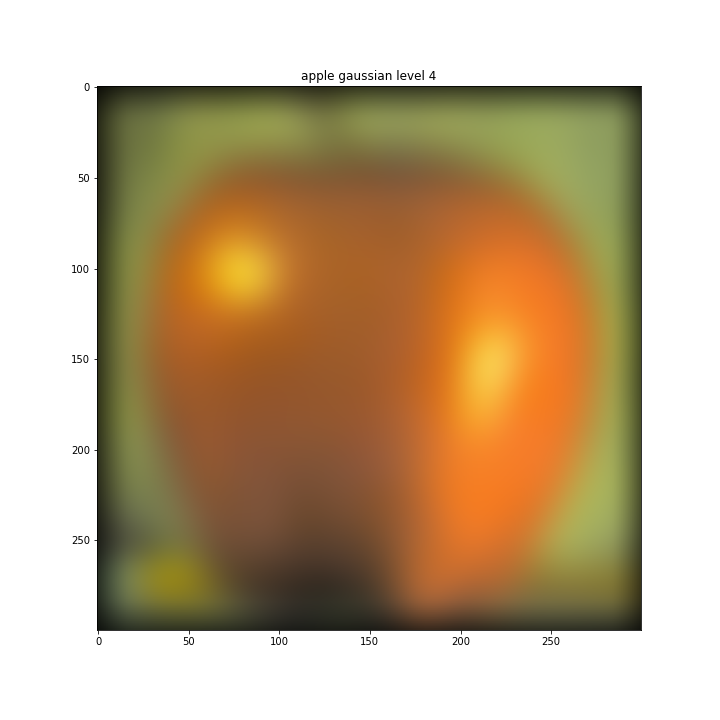
\includegraphics[width=\linewidth]{apple gaussian level 4.png}
\endminipage
\end{figure}

\begin{figure}[!htb]
\title{apple laplacian}
\minipage{0.24\textwidth}
    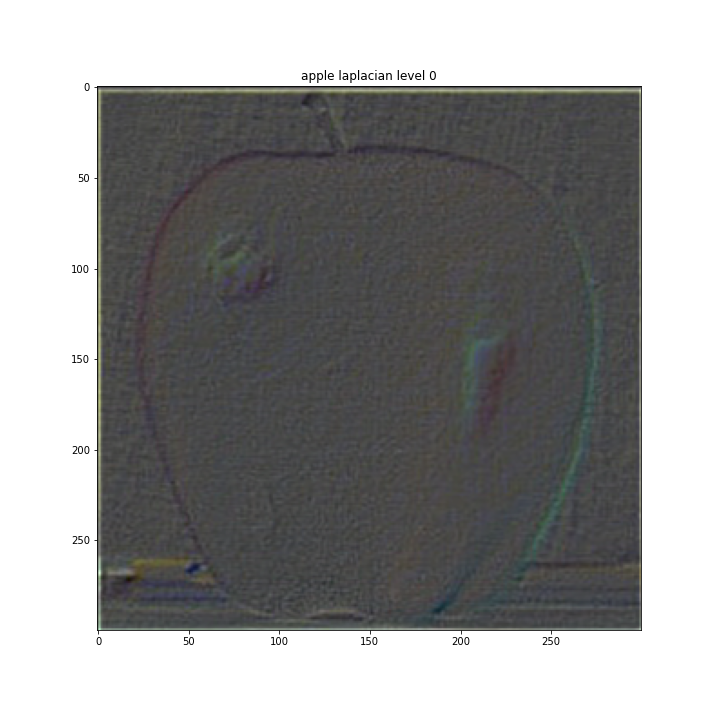
\includegraphics[width=\linewidth]{apple laplacian level 0.png}
\endminipage
\minipage{0.24\textwidth}
    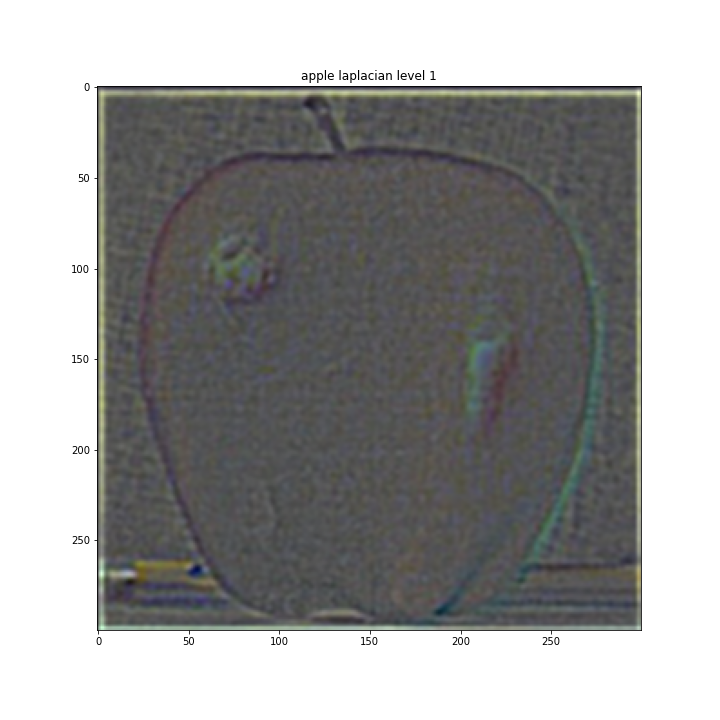
\includegraphics[width=\linewidth]{apple laplacian level 1.png}
\endminipage
\minipage{0.24\textwidth}
    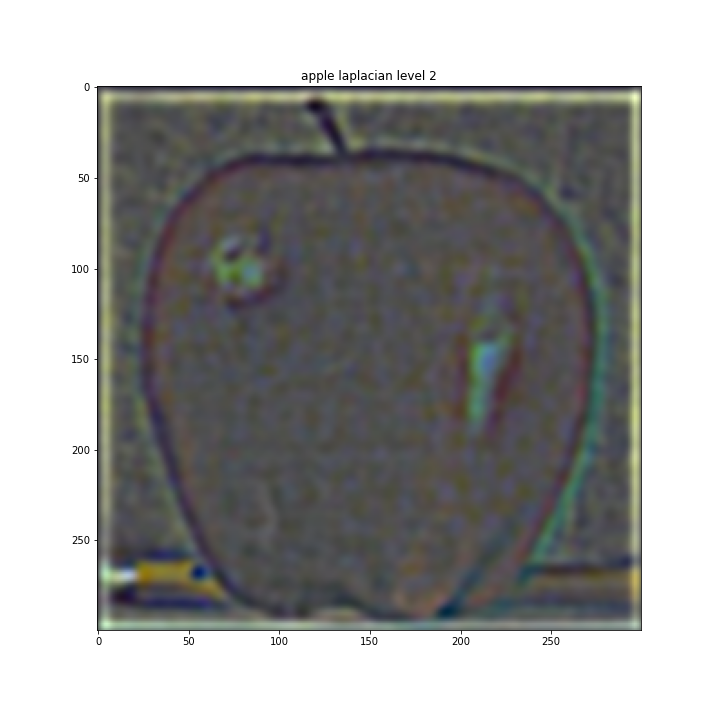
\includegraphics[width=\linewidth]{apple laplacian level 2.png}
\endminipage
\minipage{0.24\textwidth}
    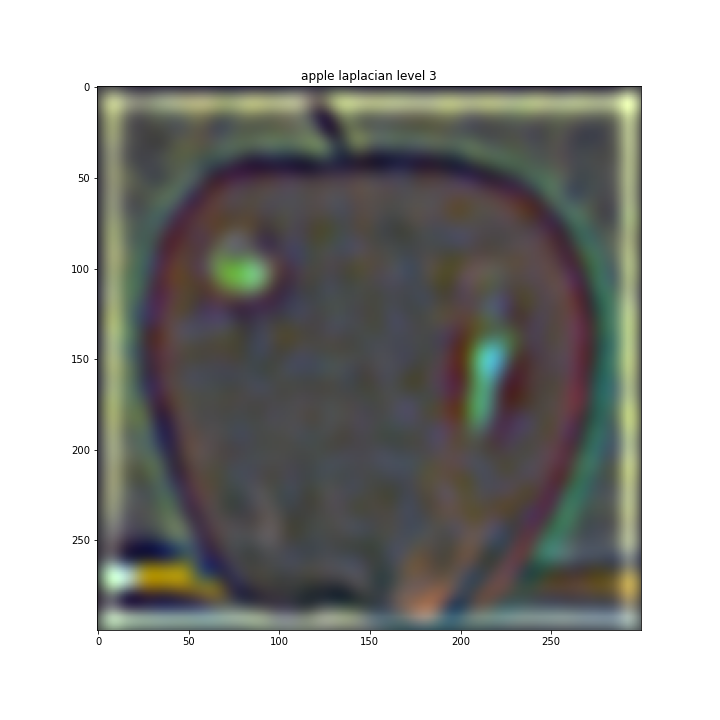
\includegraphics[width=\linewidth]{apple laplacian level 3.png}
\endminipage
\minipage{0.24\textwidth}
    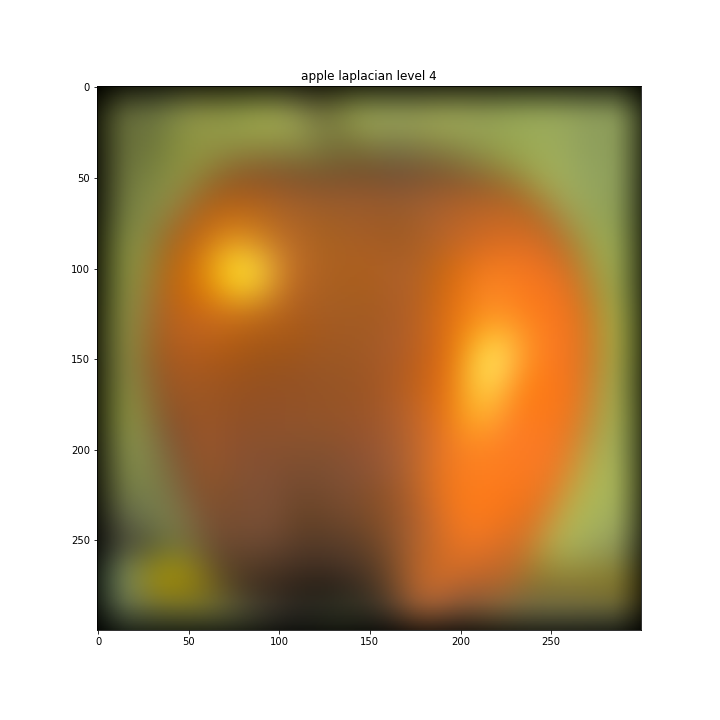
\includegraphics[width=\linewidth]{apple laplacian level 4.png}
\endminipage
\end{figure}

\begin{figure}[!htb]
\title{orange gaussian}
\minipage{0.24\textwidth}
    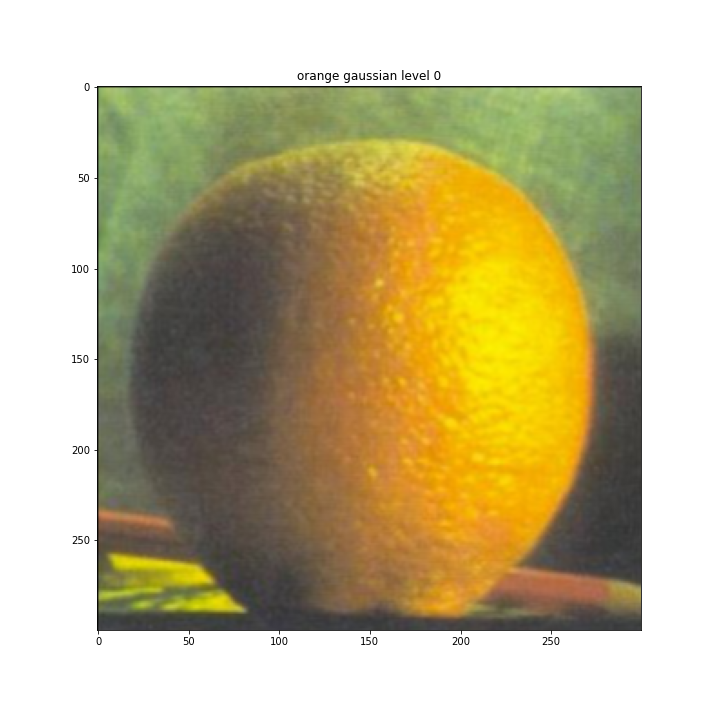
\includegraphics[width=\linewidth]{orange gaussian level 0.png}
\endminipage
\minipage{0.24\textwidth}
    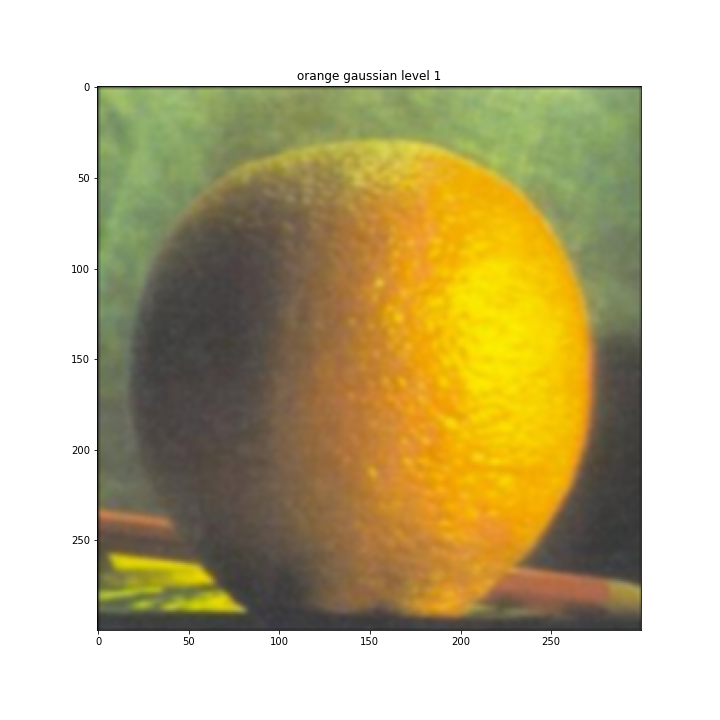
\includegraphics[width=\linewidth]{orange gaussian level 1.png}
\endminipage
\minipage{0.24\textwidth}
    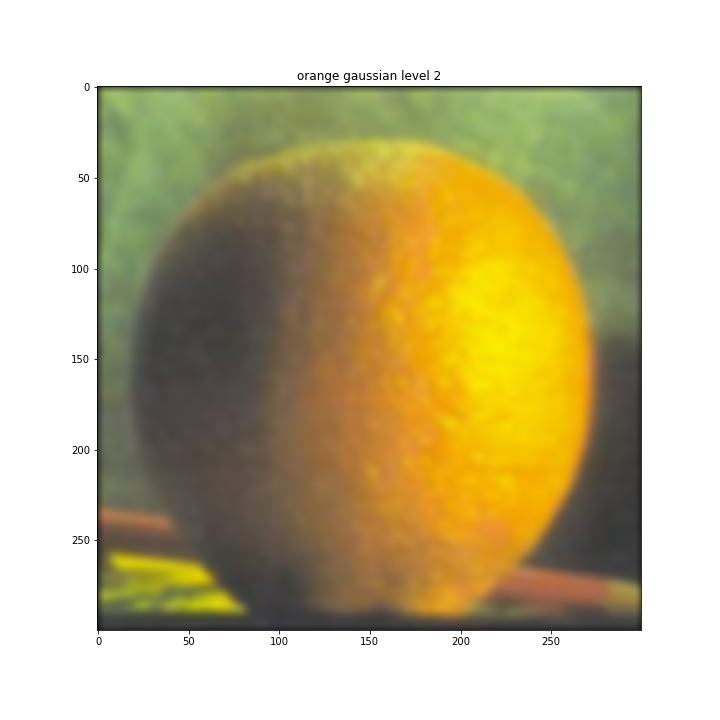
\includegraphics[width=\linewidth]{orange gaussian level 2.png}
\endminipage
\minipage{0.24\textwidth}
    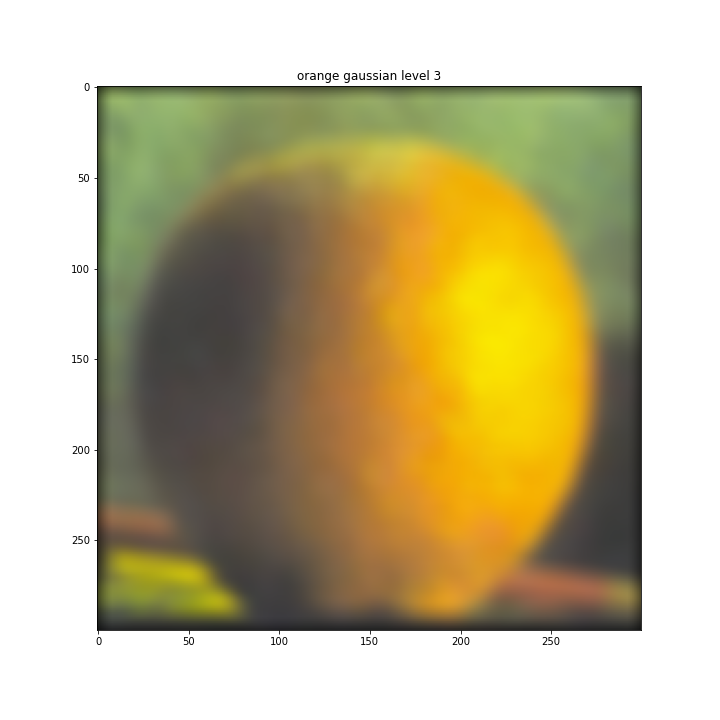
\includegraphics[width=\linewidth]{orange gaussian level 3.png}
\endminipage
\minipage{0.24\textwidth}
    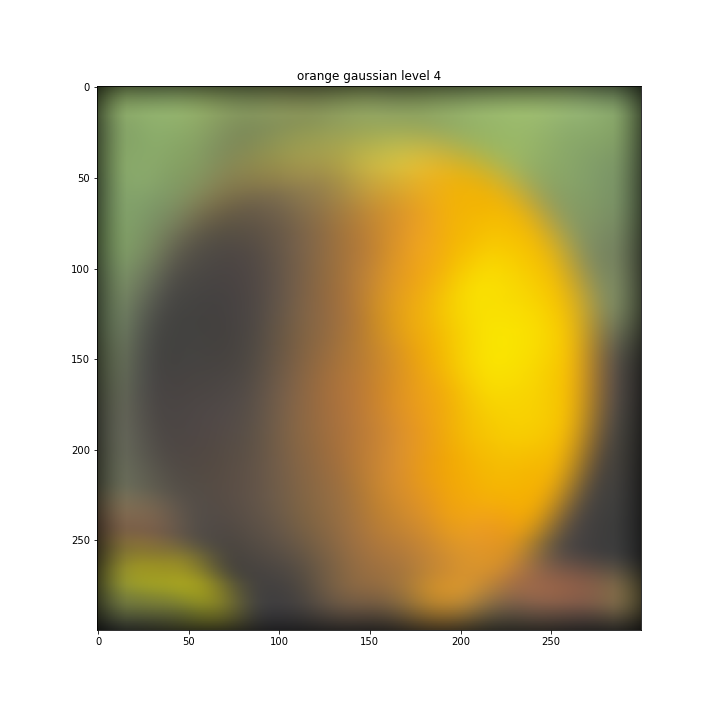
\includegraphics[width=\linewidth]{orange gaussian level 4.png}
\endminipage
\end{figure}

\begin{figure}[!htb]
\title{orange laplacian}
\minipage{0.24\textwidth}
    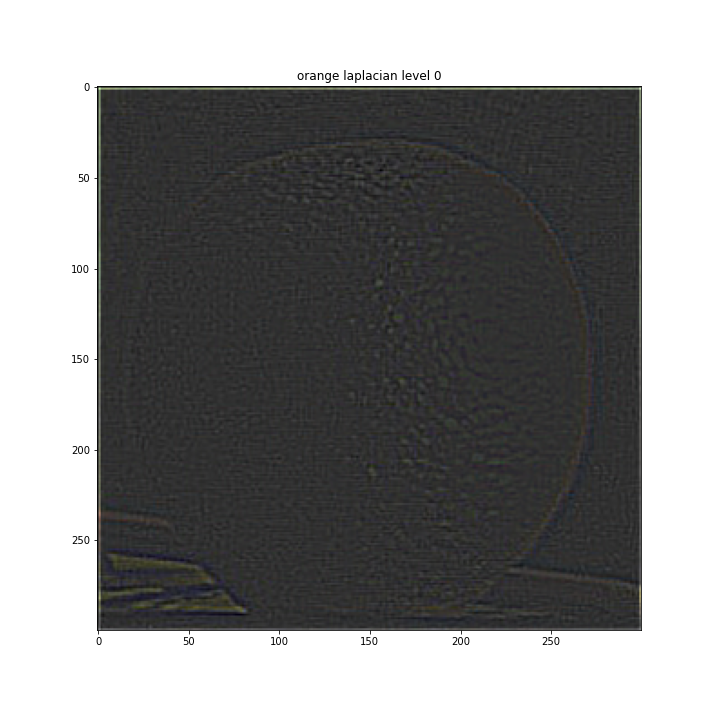
\includegraphics[width=\linewidth]{orange laplacian level 0.png}
\endminipage
\minipage{0.24\textwidth}
    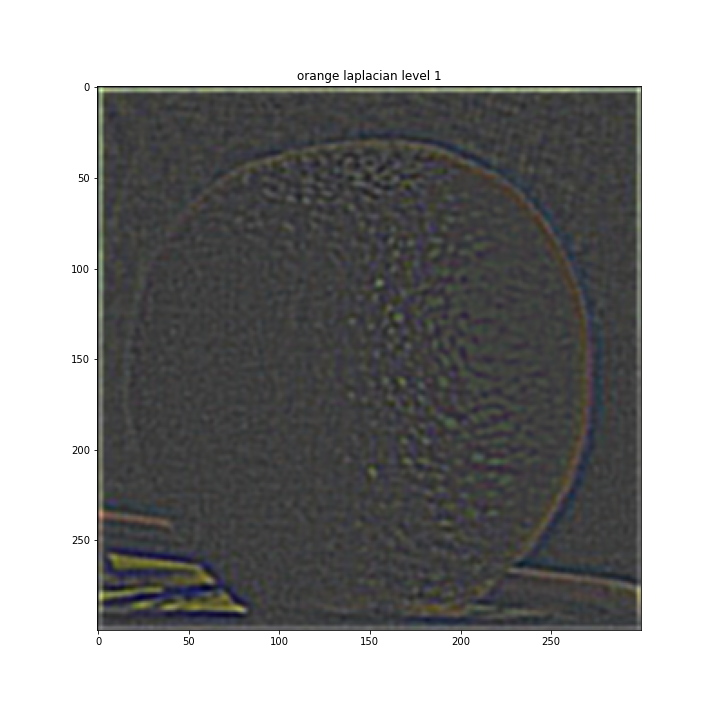
\includegraphics[width=\linewidth]{orange laplacian level 1.png}
\endminipage
\minipage{0.24\textwidth}
    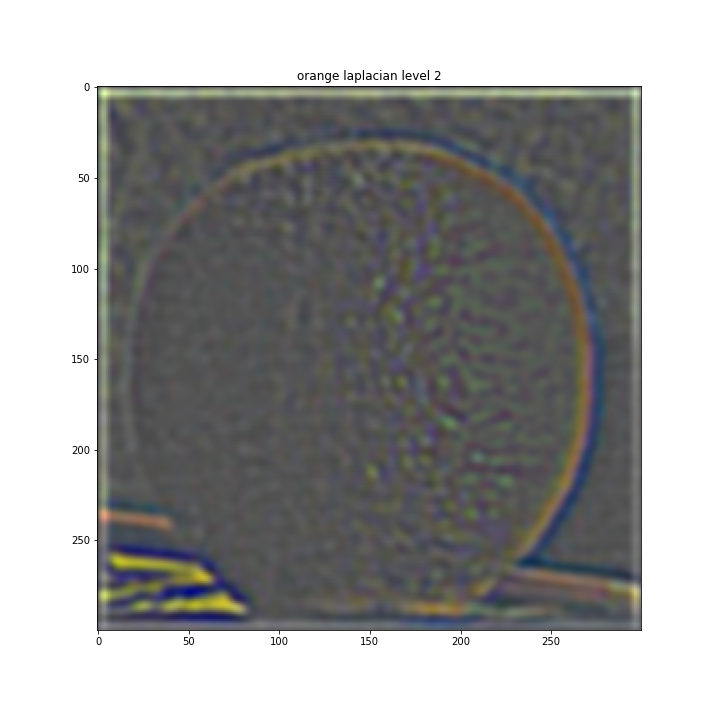
\includegraphics[width=\linewidth]{orange laplacian level 2.png}
\endminipage
\minipage{0.24\textwidth}
    \includegraphics[width=\linewidth]{orange laplacian level 3.png}
\endminipage
\minipage{0.24\textwidth}
    \includegraphics[width=\linewidth]{orange laplacian level 4.png}
\endminipage
\end{figure}
\FloatBarrier

\title{Re-creating Figure 3.42}
\begin{figure}[!htb]
\title{level 0}
\minipage{0.35\textwidth}
    \includegraphics[width=\linewidth]{LHS 0.png}
    \caption{LHS}
\endminipage
\minipage{0.35\textwidth}
    \includegraphics[width=\linewidth]{RHS 0.png}
    \caption{RHS}
\endminipage
\minipage{0.35\textwidth}
    \includegraphics[width=\linewidth]{blended laplacian level 0.png}
    \caption{LHS+RHS}
\endminipage
\end{figure}

\begin{figure}[!htb]
\title{level 2}
\minipage{0.35\textwidth}
    \includegraphics[width=\linewidth]{LHS 2.png}
    \caption{LHS}
\endminipage
\minipage{0.35\textwidth}
    \includegraphics[width=\linewidth]{RHS 2.png}
    \caption{RHS}
\endminipage
\minipage{0.35\textwidth}
    \includegraphics[width=\linewidth]{blended laplacian level 2.png}
    \caption{LHS+RHS}
\endminipage
\end{figure}

\begin{figure}[!htb]
\title{level 4}
\minipage{0.35\textwidth}
    \includegraphics[width=\linewidth]{LHS 4.png}
    \caption{LHS}
\endminipage
\minipage{0.35\textwidth}
    \includegraphics[width=\linewidth]{RHS 4.png}
    \caption{RHS}
\endminipage
\minipage{0.35\textwidth}
    \includegraphics[width=\linewidth]{blended laplacian level 4.png}
    \caption{LHS+RHS}
\endminipage
\end{figure}

\begin{figure}[!htb]
\title{collapsed}
\minipage{0.35\textwidth}
    \includegraphics[width=\linewidth]{LHS recreated.png}
    \caption{LHS}
\endminipage
\minipage{0.35\textwidth}
    \includegraphics[width=\linewidth]{RHS recreated.png}
    \caption{RHS}
\endminipage
\minipage{0.35\textwidth}
    \includegraphics[width=\linewidth]{orapple.png}
    \caption{LHS+RHS}
\endminipage
\end{figure}
\FloatBarrier

\subsection{Multiresolution Blending}

\title{Liger Eyes}
\begin{figure}[!htb]
\minipage{0.50\textwidth}
    \includegraphics[width=\linewidth]{lionface.jpeg}
    \caption{LHS}
\endminipage
\minipage{0.50\textwidth}
    \includegraphics[width=\linewidth]{tigerface.jpg}
    \caption{RHS}
\endminipage
\end{figure}

\begin{figure}[!htb]
\minipage{0.45\textwidth}
    \includegraphics[width=\linewidth]{liger_mask.png}
    \caption{Mask}
\endminipage
\minipage{0.65\textwidth}
    \includegraphics[width=\linewidth]{liger.png}
    \caption{Collapsed}
\endminipage
\end{figure}

\title{Irregular Mask–New President}
\begin{figure}[!htb]
\minipage{0.50\textwidth}
    \includegraphics[width=\linewidth]{trump.jpg}
    \caption{Base}
\endminipage
\minipage{0.50\textwidth}
    \includegraphics[width=\linewidth]{obamaface.png}
    \caption{Blend In}
\endminipage
\end{figure}

\begin{figure}[!htb]
\minipage{0.45\textwidth}
    \includegraphics[width=\linewidth]{president_mask.png}
    \caption{Mask}
\endminipage
\minipage{0.65\textwidth}
    \includegraphics[width=\linewidth]{mypresident.png}
    \caption{Collapsed}
\endminipage
\end{figure}
\FloatBarrier

\section{Reflection}
This was really cool. I've played around with photoshop before, but I never knew it was using a bunch of math. The hard part was finding images that would align correctly.

\end{document}
